\documentclass{beamer}

\usepackage{graphicx}
\usepackage{listings}

\mode<presentation>

\title{Diving into Flask}

\author[A. Mishkovskyi]{Andrii V. Mishkovskyi \\ \texttt{contact@mishkovskyi.net}}
\date[EuroPython 2012]

\begin{document}

\lstset{
  language=Python,
  basicstyle=\ttfamily,
  columns=fixed,
  showspaces=false,
  showstringspaces=false,
}

\section{Introduction}

% Or should I do a "this guy" text + an arrow pointing to me?

\begin{frame}{Who am I?}
  \begin{itemize}
  \item Developer for Hyves
  \item Python fan
  \item Heavy user of Flask (and Werkzeug in the past)
  \end{itemize}
\end{frame}

\begin{frame}{What is Hyves?}
  \begin{itemize}
  \item The 2nd biggest social network in Netherlands
  \item Used to be exclusively PHP shop
  \item Primarily Python nowadays
  \item And primarily Flask
  \end{itemize}
\end{frame}

\begin{frame}
  \frametitle{Why Flask?}
  \only<1>{
    \begin{itemize}
    \item Well-documented
    \item Great API
    \item Easily extendable
    \end{itemize}
  }
  \only<2>{
    \begin{center}
      \LARGE{Yes, we also considered Django, Pyramid and many more}
    \end{center}
  }
\end{frame}

\begin{frame}
  \frametitle{Presentation theme}
  \begin{itemize}
  \item Share our experience with Flask
  \item Explore inner workings of some features
  \item Understand why things break
  \end{itemize}
\end{frame}

\section{Exploring Flask}

\subsection{Starting with the simplest}

\begin{frame}[fragile]
  \frametitle{This is where you start}
  \only<1>{
    \lstinputlisting[language=Python]{code/simplest.py}
  }
  \only<2>{
    \lstinputlisting[language=Python,lastline=6,firstline=4]{code/simplest.py}
  }
\end{frame}

\subsection{Simple, yet powerful}

\begin{frame}
  \frametitle{\texttt{Flask.route}}
  \begin{itemize}
  \item Decorator that calls \texttt{Flask.add\_url\_rule}
  \item \texttt{Flask.add\_url\_rule} creates \texttt{werkzeug.routing.Rule}
    and adds it to \texttt{werkzeug.routing.Map}
  \item \texttt{werkzeug.routing.Map} does the URL matching magic
  \end{itemize}
\end{frame}

\begin{frame}
  \frametitle{URL matching and decomposition}
  \only<1>{
    \begin{itemize}
    \item \texttt{Rule} creates regexp and collects proper converters
    \item \texttt{Map} holds all rules and builds the string for Rule to match
    \item \texttt{Converter}s convert the path parts into Python objects
    \end{itemize}
  }
  % Flask also tries to save some time matching URLs and sorts
  % Rules in specific order, see the key function for Rule
  \only<2>{\lstinputlisting{code/flask-routing-example.py}}
  \only<3>{\texttt{Rule}s are stored in \texttt{Map} in sorted order.
    \lstinputlisting{code/flask-routing-rule-order.py}}
\end{frame}

\subsection{Flask views}

\begin{frame}
  \frametitle{Manual dispatch}
  \lstinputlisting{code/flask-routing-manual-dispatch.py}
\end{frame}

\begin{frame}
  \frametitle{Let Flask do all the hard work}
  \lstinputlisting{code/flask-routing-function-level.py}
\end{frame}

\begin{frame}
  \frametitle{Class views? No problem!}
  \lstinputlisting{code/flask-routing-class-based.py}
\end{frame}

\subsection{Blueprints}

\begin{frame}
  \frametitle{Modular Flask}
  \begin{itemize}
  \item More manageable
  \item No more interference with other's work
  \item Turnkey functionality implementations
  \end{itemize}
\end{frame}

\begin{frame}
  \frametitle{Introducing blueprints}
  \begin{itemize}
  \item We needed API versioning
  \item Instant win: \texttt{url\_prefix}
  \item
  \end{itemize}
\end{frame}

\begin{frame}
  \frametitle{How do blueprints work}
  \begin{itemize}
  \item
  \end{itemize}

\end{frame}

\section{Flask and SQLAlchemy}

\subsection{Overview}

\begin{frame}
  \frametitle{Flask SQLAlchemy}
  flask-sqlalchemy
  apply\_driver\_hacks
\end{frame}

\subsection{Partitioning}

\begin{frame}
  \frametitle{SQLAlchemy and binds}
\only<1>{
  \begin{itemize}
  \item Bind is the engine SQLAlchemy uses
  \item Flask-SQLAlchemy gives the ability to specify the bind for each model
  \end{itemize}
}
\only<2>{
  \lstinputlisting{code/flask-sqlalchemy-bind-example.py}
}
\end{frame}

\begin{frame}
  \frametitle{Flask-SQLAlchemy subclasses sqlalchemy.Session}
  \lstinputlisting{code/flask-sqlalchemy-binds.py}
\end{frame}

\begin{frame}
  \frametitle{How do we achieve master-slave support?}
  \only<1>{
    \lstinputlisting[lastline=8]{code/flask-sqlalchemy-select-bind-explicitely.py}}
  \only<2>{
    \lstinputlisting[firstline=10,lastline=17]{code/flask-sqlalchemy-select-bind-explicitely.py}}
  \only<3>{
    \lstinputlisting[firstline=18]{code/flask-sqlalchemy-select-bind-explicitely.py}}
  \only<4>{
    \lstinputlisting{code/flask-sqlalchemy-bind-selection.py}
  }
\end{frame}

\subsection{Migrations}

\begin{frame}
  \frametitle{SQLAlchemy-migrate}
  \texttt{http://sqlalchemy-migrate.readthedocs.org/}
  \begin{itemize}
  \item Easy to start with
  \item Decent documentation
  \item Seems abandoned
  \item Had to write a wrapper to run \texttt{migrate} utility
  \end{itemize}
\end{frame}

\begin{frame}
  \frametitle{Alembic}
  \texttt{http://alembic.readthedocs.org/}
  \begin{itemize}
  \item 7 months ago seemed to be in alpha state
  \item Much more mature right now
  \item Great documentation, great implementation
  \item Written by Mike Bayer himself
  \end{itemize}
\end{frame}

\section{Deferring your tasks}

\subsection{Introducing celery}

\begin{frame}
  \frametitle{Celery features}
  \begin{itemize}
  \item Removes the hassle of using amqplib/pika
  \item Extensive set of features
  \item Confusing documentation
  \end{itemize}
\end{frame}

\begin{frame}
  \frametitle{Flask-Celery}
  \only<1>{
    \begin{itemize}
    \item You have to use Flask-Script
    \item Most of the commands work
    \item Except for starting detached celery daemons
    \end{itemize}
  }
  \only<2>{\lstinputlisting{code/flask-celery-detached.py}}
\end{frame}


\subsection{Celery and logging}

\begin{frame}
  \frametitle{Color formatting}
  \begin{block}{Problem}
    Celery always resorts to ColorFormatter. We don't like colors.
  \end{block}
  \begin{block}{Solution}
    Add \texttt{after\_setup\_logger} signal that reassigns all
    logging formatters for Celery.
  \end{block}
\end{frame}

\begin{frame}
  \frametitle{OH HEY COLORZ}
  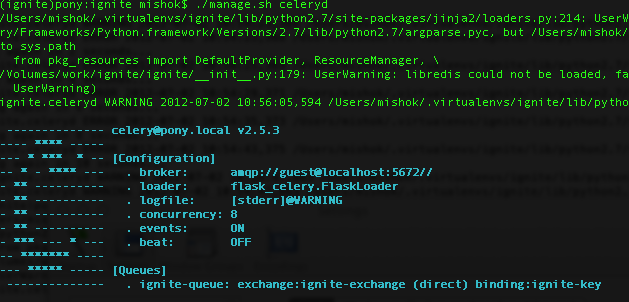
\includegraphics[scale=0.5]{images/celery-colored.png}
\end{frame}

\begin{frame}
  \frametitle{Hijacking root logger}
  \begin{block}{Problem}
    Root logger is hijacked by Celery's logging setup, making your logging
    setup useless.
  \end{block}
  \begin{block}{Solution}
    Set \texttt{CELERYD\_HIJACK\_ROOT\_LOGGER} to \texttt{False}. Or better
    yet, never use root logger.
  \end{block}
\end{frame}

\begin{frame}
  \frametitle{Process name}
  \begin{block}{Problem}
    Logging might brake if you want to setup logging beyond log message
    format.
  \end{block}
  \begin{block}{Solution}
    See \texttt{https://gist.github.com/721870}
    \begin{quotation}
      There are three places in the code where the processName is written to a
      LogRecord, some of which can lead to unexpected behaviour in some scenarios
  \end{quotation}
  \end{block}
\end{frame}

\subsection{Monitoring Celery}

% https://github.com/celery/django-celery/blob/master/djcelery/snapshot.py

\begin{frame}
  \frametitle{Take a look inside}
\only<1-2>{  \begin{itemize}
  \item Subclass \texttt{celery.events.snapshot.Polaroid}
    \only<1>{
    \item ???
    \item PROFIT
    }
    \only<2>{
    \item Write \texttt{on\_shutter} method
    \item Check various metrics
    \item Generate report in whatever format you need
    }
  \end{itemize}
}
\only<3>{
  \lstinputlisting{code/celery-polaroid.py}
}
\end{frame}

\subsection{Celery and Flask-SQLAlchemy}

\begin{frame}
  \frametitle{Celery + SQLAlchemy + MySQL}
  \only<1>{
    \begin{block}{Problem}
      Each time worker starts, infamous error is raised:
      \begin{quotation}
        OperationalError:\\
        (2006, 'MySQL server has gone away')
      \end{quotation}
    \end{block}
    \begin{block}{Solution}
      Drop the whole connection (engine) pool at worker init.
    \end{block}
  }
  \only<2>{
    \lstinputlisting{code/celery-drop-sqlalchemy-connections.py}
  }
  \only<3>{
    \begin{block}{Problem}
      Session not closed if exception happens middle-way through
    \end{block}
    \begin{block}{Solution}
      Close the session in \texttt{task\_postrun} signal.
    \end{block}
  }
  \only<4>{
    \lstinputlisting{code/celery-close-session-unconditionally.py}
  }
  \only<5>{
    \begin{block}{Problem}
      Session still not closed properly if \alert{db object loses app context}.
      Worker hangs too if that happens.
      \begin{quotation}
        RuntimeError: application not registered on db instance
        and no application bound to current context
      \end{quotation}
    \end{block}
    \begin{block}{Solution}
      Close the session in \texttt{task\_postrun} signal \alert{but only
        if there was an exception}.
    \end{block}
  }
  \only<6>{
    \lstinputlisting{code/celery-close-session-unconditionally-proper.py}
  }
\end{frame}

\section{Other niceties}

\subsection{Caching}

\begin{frame}
  \frametitle{Flask-Cache}
  \begin{itemize}
  \item More focused on caching views
  \item Quite a few caching decorators
  \item Otherwise -- thin wrapper around werkzeug.contrib.cache
  \end{itemize}
\end{frame}

\begin{frame}
  \frametitle{But we're special!}
  \begin{itemize}
  \item Wrote our own cache classes
  \item With namespace support
  \item And consistent hashing (libketama + libredis)
  \end{itemize}
\end{frame}

\subsection{Profiling}

\begin{frame}
  \frametitle{Profiling}
\end{frame}

\section*{Conclusion}

\begin{frame}
  \frametitle{Flask maturity}
  \begin{itemize}
  \item Flask is no longer an April Fool's joke
  \item Still micro, but not in terms of features
  \item You can and should build applications with Flask
  \item Flask is easy to reason about
  \end{itemize}
\end{frame}

\begin{frame}
  \frametitle{Flask's ecosystem}
  \begin{itemize}
  \item Not on par with Flask in places
  \item Interoperability is rough in places
  \item Lack's BDFL for extensions (mitsuhiko for president!)
  \end{itemize}
\end{frame}

\begin{frame}
  \frametitle{Questions?}
\end{frame}

\end{document}

%% Diving into Flask (Head On)

Intro

What we've built

Based on our experience with social networks and pressing necessity
in integrating with other social networks, we have decided to create
a unifying API. It's similar to Janrein, Gigya and Spring Social in many
ways, but being built in-house gives us some advantages over 3rd party
solutions (read: MONEY)
We have strict requirements in terms of availability and speed of
development.

Decision for Flask

Flask started as an April's Fool joke, but look who's laughing now. Armin's not
laughing, because he has to support it nowadays. But seriously, Flask is a very
mature project nowadays and provides you with everything you need to
modern build web applications. SQLAlchemy, no template needs, etc made flask
a better option than Django.

Flask's tutorial starts with a minimal example of an application
Even though it looks nice, don't be fooled by it -- you're likely to
grow out of one file as soon as you start putting real functionality
into your application. But Flask doesn't stop being useful at this stage
unlike some other frameworks (I'm looking at you, web.py). Flask has all
the the required functionality to grow into enterprise level (sarcasm intended)

Flask's REST support is great. Here you go:
...
You can also have class views (I'm not sure what's the latest Django view on those)
...

But what if you want to use Flask from JavaScript? Well, you either have to
build your own dispatcher, or use _method trick:
...

But how does that work? Let's first dive a bit into how Werkzeug builds routes
(after all it's werkzeug doing the actual route dispatch work):
...
As you can see, the last step is to build regexp and then matching an endpoint
But how does method plays in here?

...

This is how you match a method. What if we want the POST handler
to react to GET request based on a certain parameter. Flask makes it easy
by using ``_method'' parameter:

...

Which translates to the following Werkzeug execution

TODO: init_app() and extensions creation
TODO: explain exthook and ext directory


Now, most application will move on to having a proper template system,
but we never needed that (except for admin) so I'm just going to skip
straight to examining Celery. After all, the whole template thing is
just plain simple.

So, Celery. Celery's great at abstracting away from all the nitty gritty
AMQP details. Well, not only AMQP, but you have to be batshit crazy to
actually anything else, right? Wrong. Anyway, Celery does AMQP and a bunch
of other backends, but our main focus here is how Flask-Celery actually works

The whole Celery deserves its own talk, so vast and mostly unexplored it is.
But we're going to take a look at how Flask-Celery achieves things

...

As we can see, there's not much to see, actually. Most of the code is
responsible for creating proper commands for the app. If you have experience
with Celery you'll note the lack of some commands, such as
celeryd_detached.


Celery also lack the init_app mechanism, which bites you in the back
as soon as you do something like this:
... show how you can't use tasks before app is initialized

Fortunately, there's a fix for that, we don't use it though (but trust me,
it works!):
https://github.com/ask/flask-celery/pull/15

But that's all nothing, we're not doing anything interesting yet.
In general most tasks will be quite straightforward

Monitoring

Logging

celeryd_detached

SQLAlchemy and flask

Flask is so minimal, that even

Flask-SQLAlchemy gives you all the things you need, but how does it work?
The binds for each model



%% celery

%% how celery behaves with various

%% celery lack of init_app

%% celery logging -- color formatting, hijacking root logger


%% detaching celery

%% sqlalchemy and celery -- issues with pool (INVESTIGATE!!! postgres too)

%% flask URL routing with RESTful interfaces

%% reading forms is slow

%% batching API -- how we did it

%% sqlalchemy flask -- indices

%% sqlalchemy migrate -- how to

%% logging -- how to

%% blueprints -- awesome

%% caching -- werkzeug.contrib.cache and consistent hashing


%% werkzeug routing -- how routes are compiled and methods checked

%% filter and validate URL parameters

%% uwsgi scaling (also talk about gunicorn)

%% werkzeug profiler, flask-debugtoolbar
%% memory?
%% cache profiling?
%% statsd integration
%% (Sentry also?)
